\documentclass[10pt,letterpaper]{article}
\usepackage[lmargin=2.2in,rmargin=0.7in,tmargin=1.0in,bmargin=1.0in]{geometry}
\usepackage{notes}
\begin{document}

\begin{center}
\Large\textbf{2.6 -- Method of Undetermined Coefficients}\\
\normalsize (Section 2.3.1)
\end{center}

%-------------------------------------------------------------
\section{Method of Undetermined Coefficients}

\subsection{Homogeneous vs. Nonhomogeneous}

So far, we have been solving \textbf{homogeneous problems} (HP):
\begin{equation}
ax''+bx'+cx=0. \tag{HP}
\end{equation}
Homogeneous means that the right-hand side is zero. A
\textbf{nonhomogeneous problem} (NHP) has the form
\begin{equation}
ax''+bx'+cx=f(t), \tag{NHP}
\end{equation}
where $f(t)$ is not identically zero. The function $f(t)$ is
called the \textbf{forcing term} or \textbf{source term}.
For a spring-mass system, it represents an external force
acting on the mass. Our goal is to solve nonhomogeneous equations
for certain types of forcing terms. We begin with a
first-order example.

%-------------------------------------------------------------
\subsection{First-Order NHP}

Consider the equation
\[
x'+2x=9e^t.
\]
We already know how to solve this using an integrating factor.
With $\mu(t)=e^{2t}$, we obtain
\begin{align*}
x(t)
&=e^{-2t}\left(\int 9e^{3t}\,dt+C\right)\\
&=e^{-2t}\left(3e^{3t}+C\right)\\
&=Ce^{-2t}+3e^t.
\end{align*}
Notice that the solution has two pieces:
\[
x(t)=
\underbrace{Ce^{-2t}}_{\text{solves }x'+2x=0}
+
\underbrace{3e^t}_{\text{solves }x'+2x=9e^t}.
\]
We will use this structure to develop a new method.

%-------------------------------------------------------------
\subsection{New Method}

We solve the same equation by finding these two pieces
separately:
\[
x(t)=x_h(t)+x_p(t).
\]
Here, $x_h$ is the \textbf{general homogeneous solution},
and $x_p$ is a \textbf{particular solution}: any one
solution of the nonhomogeneous equation.

\paragraph{Step 1. Find the homogeneous solution.}
Temporarily set the forcing term to zero:
\[
x'+2x=0.
\]
The general solution is
\[
x_h(t)=Ce^{-2t}.
\]

\paragraph{Step 2. Choose a trial function.}
Since the forcing term is $9e^t$, we guess a form for the particular solution
\[
x_p(t)=Ae^t,
\]
where $A$ is an unknown coefficient. Differentiating $e^t$
preserves its form, so this is a reasonable guess.

\paragraph{Step 3. Determine the coefficient.}
Substitute the trial function into the nonhomogeneous equation:
\begin{align*}
x_p'+2x_p&=9e^t\\
Ae^t+2Ae^t&=9e^t\\
3Ae^t&=9e^t.
\end{align*}
Thus, $A=3$ and $x_p(t)=3e^t$.

\paragraph{Step 4. Combine the two pieces.}
The general solution is
\[
\boxed{x(t)=x_h(t)+x_p(t)=Ce^{-2t}+3e^t.}
\]
This agrees with the integrating-factor solution.
The same approach also works for second-order equations.

%-------------------------------------------------------------
\subsection{Why the Sum Works}
Why does the summation 
$$
    x=x_h+x_p
$$
work?
Suppose $x_h$ solves the homogeneous equation and $x_p$
solves the nonhomogeneous equation. Substituting their sum gives
\begin{align*}
ax''+bx'+cx&=f(t)\\
a(x_h+x_p)''+b(x_h+x_p)'+c(x_h+x_p)&=f(t)\\
(ax_h''+bx_h'+cx_h)+(ax_p''+bx_p'+cx_p)&=f(t)\\
(0)+(f(t))&=f(t)\\
f&=f \; \checkmark
\end{align*}
Therefore, $x_h+x_p$ solves the nonhomogeneous equation. This is basis of a techniuqe called the \textit{method of undetermined coefficients.}

%-------------------------------------------------------------
\subsection{Method of Undetermined Coefficients}

The \textbf{method of undetermined coefficients} finds a
particular solution by choosing a trial function with unknown
coefficients and solving for them. To solve
\[
ax''+bx'+cx=f(t),
\]
use the following steps:
\begin{enumerate}
    \item Find the general homogeneous solution $x_h$ by solving
    \[
    ax''+bx'+cx=0.
    \]

    \item Choose a trial function for $x_p$ based on the form
    of $f(t)$. 

    \item Substitute $x_p$ into the nonhomogeneous equation
    and solve for its unknown coefficients.

    \item Write the general solution
    \[
    x(t)=x_h(t)+x_p(t).
    \]

    \item If initial conditions are given, apply them to the
    complete solution to determine the arbitrary constants.
\end{enumerate}

We already know how to find $x_h$ using the characteristic
equation. The new task is choosing a suitable trial function
for $x_p$, which we discuss next. 



%%%%%%%%%%%%%%%%%%%%%%%%%%%%%%%%%%%%%%%%%%%%%%%%%%%%%%%%%%%%%%%%%%%%%%%%
\section{The Trial Function}

\subsection{When the Method Applies}

The method of undetermined coefficients applies when the forcing
term $f(t)$ is built from:
\begin{itemize}
    \item Polynomials,
    \item Exponentials $e^{\beta t}$,
    \item Waves $\sin(\omega t)$ and $\cos(\omega t)$,
    \item Sums and products of these functions.
\end{itemize}
For example, we can use the method to solve
\[
x''+x'+x=3e^{2t}\sin t+t^2,
\]
but it does not apply to
\[
x''+x'+x=\ln t.
\]
The key feature of the allowed functions is that repeated
differentiation produces the same types of terms. This lets
us choose a trial function with finitely many unknown coefficients.

%-------------------------------------------------------------
\subsection{Table of Trial Functions}

The table below gives the basic trial forms. Greek letters
represent known constants from the forcing term; capital
Latin letters represent unknown coefficients.

\begin{table}[H]
\centering
\renewcommand{\arraystretch}{1.6}
\begin{tabular}{|c|c|c|}
\hline
\textbf{Type}
& \textbf{Forcing term $f(t)$}
& \textbf{Trial function $x_p(t)$}\\
\hline
Constant
& $\alpha$
& $A$\\
\hline
Exponential
& $\alpha e^{\beta t}$
& $Ae^{\beta t}$\\
\hline
Polynomial
& $\alpha_2t^2+\alpha_1t+\alpha_0$
& $At^2+Bt+C$\\
\hline
Wave
& \shortstack{$\alpha\sin(\omega t)$ or $\alpha\cos(\omega t)$}
& $A\cos(\omega t)+B\sin(\omega t)$\\
\hline
\end{tabular}
\caption{Basic trial forms before checking for duplication
with the homogeneous solution.}
\end{table}

The polynomial row extends to any degree: for a polynomial
of degree $n$, use a trial polynomial of degree $n$ with an
unknown coefficient for every power of $t$, including the constant. 
These are \textbf{initial trial forms}. If a trial overlaps
with the homogeneous solution, we must modify it using the
duplicate rule introduced in the next section.

%-------------------------------------------------------------
\begin{example}[1]{
Find an initial trial function for each forcing term,
before checking for duplication.
\begin{enumerate}
    \item $f(t)=6$
    \item $f(t)=-3e^{4t}$
    \item $f(t)=3t^2$
    \item $f(t)=12\sin 3t$
\end{enumerate}
}
\begin{enumerate}
    \item For a constant forcing term, try
    \[
    x_p(t)=A.
    \]

    \item For an exponential forcing term, keep the
    same exponent:
    \[
    x_p(t)=Ae^{4t}.
    \]

    \item For a quadratic forcing term, include every
    power through degree two:
    \[
    x_p(t)=At^2+Bt+C.
    \]

    \item For a sinusoidal forcing term, include both
    sine and cosine with the same frequency:
    \[
    x_p(t)=A\cos 3t+B\sin 3t.
    \]
\end{enumerate}
\end{example}

The trial function may need terms that are absent from $f(t)$.
Our goal is to include the types of terms produced by
differentiation. For example, if $f(t)=3t^2$, we use
\[
x_p(t)=At^2+Bt+C,
\]
even though the forcing term has no linear or constant term.
Including all three coefficients gives us the freedom to
match the quadratic term and cancel any unwanted lower-degree
terms after substitution. The same goes for waves. We need both 
the sine and cosine because their derivatives switch between the two. 

Now we are ready for a second-order problem.

% -------------------------

\begin{example}[2]{
Find the general solution to
\[
x''-3x'+2x=2t^2-3.
\]
}
First, solve the homogeneous equation. The characteristic equation is
\[
\lambda^2-3\lambda+2=(\lambda-1)(\lambda-2)=0,
\]
so
\[
x_h(t)=c_1e^t+c_2e^{2t}.
\]

Since the forcing term is a quadratic polynomial, use
\[
x_p(t)=At^2+Bt+C.
\]
We include the linear term even though it does not appear
in the forcing term. Differentiating gives
\[
x_p'=2At+B,
\qquad
x_p''=2A.
\]
Substitute into the nonhomogeneous equation and collect
like powers of $t$:
\begin{align*}
2A-3(2At+B)+2(At^2+Bt+C)&=2t^2-3,\\
(2A)t^2+(2B-6A)t+(2A-3B+2C)&=2t^2-3.
\end{align*}
For this equality to hold for every $t$, the coefficients
of corresponding powers must match:
\[
\begin{dcases}
2A=2,\\
2B-6A=0,\\
2A-3B+2C=-3.
\end{dcases}
\]
Solving in order gives
\[
A=1,\qquad B=3,\qquad C=2.
\]
Therefore, $x_p(t)=t^2+3t+2$, and the general solution is
\[
\boxed{x(t)=c_1e^t+c_2e^{2t}+t^2+3t+2.}
\]
\end{example}

%%%%%%%%%%%%%%%%%%%%%%%%%%%%%%%%%%%%%%%%%%%%%%%%%%%

\section{Rules for Trial Functions}

The basic trial forms extend to more complicated forcing terms.
We use three rules: the sum rule, the product rule, and the
duplicate rule.

%-------------------------------------------------------------
\subsection{Sum Rule}

If the forcing term is a sum, add the trial forms for its
individual terms. Use separate unknown coefficients for
each part.

For example, if
\[
x''+2x=t+\sin 3t,
\]
then the initial trial function is
\[
x_p(t)=
\underbrace{At+B}_{\text{for }t}
+
\underbrace{C\cos 3t+D\sin 3t}_{\text{for }\sin 3t}.
\]
We can substitute the entire trial function at once or
find a particular solution for each forcing term separately
and add the results. For instance, you may substitute 
$$
At+B
$$
into $x''+2x=t$ and solve for $A$ and $B$. Then you can 
substitute
$$
C\cos3t+D\sin3t
$$
into $x''+2x=\sin3t$ to find $C$ and $D$. Then combine the results at the end.
%-------------------------------------------------------------
\subsection{Product Rule}

When the forcing term is a product of a polynomial, an
exponential, and a wave, combine their trial forms.
After expanding, give every distinct term its own
unknown coefficient.

\paragraph{Polynomial times exponential.}
For a forcing term such as
\[
f(t)=4te^{2t},
\]
use a full linear polynomial multiplied by the exponential:
\[
x_p(t)=(At+B)e^{2t}.
\]

\paragraph{Exponential times wave.}
For
\[
f(t)=e^{-3t}\sin 2t,
\]
include both sine and cosine:
\[
x_p(t)=e^{-3t}(A\cos 2t+B\sin 2t).
\]

\paragraph{Polynomial times wave.}
For
\[
f(t)=t\cos t,
\]
give sine and cosine their own full linear polynomials:
\[
x_p(t)=(At+B)\cos t+(Ct+D)\sin t.
\]
Do not use $(At+B)(C\cos t+D\sin t)$: that form ties
the coefficients together. The coefficients of
$t\cos t$, $\cos t$, $t\sin t$, and $\sin t$
must be independent.

%-------------------------------------------------------------
\subsection{Duplicate Rule}

Before using a trial function, compare it with the
homogeneous solution. If it contains terms already present
in $x_h$, multiply the corresponding trial group by the
smallest power of $t$ that removes the overlap. 

To see why this is necessary, consider
\[
x''-4x=e^{2t}.
\]
The homogeneous solution is
\[
x_h(t)=c_1e^{2t}+c_2e^{-2t}.
\]
Our initial guess would be $x_p(t)=Ae^{2t}$, but substituting
gives
\[
x_p''-4x_p=4Ae^{2t}-4Ae^{2t}=0.
\]
No choice of $A$ can make this equal to $e^{2t}$.
The trial function already solves the homogeneous equation.

Multiply the guess by $t$:
\[
x_p(t)=Ate^{2t}.
\]
Then
\[
x_p'=(A+2At)e^{2t},
\qquad
x_p''=(4A+4At)e^{2t}.
\]
Substituting into the nonhomogeneous equation gives
\[
x_p''-4x_p=4Ae^{2t}=e^{2t},
\]
so $A=\frac14$. Therefore,
\[
\boxed{x(t)=c_1e^{2t}+c_2e^{-2t}+\frac14te^{2t}.}
\]

%-------------------------------------------------------------
\begin{example}[3]{
Choose an appropriate trial function for each equation.
Do not solve for the coefficients.
\begin{enumerate}
    \item $x''-x=2t+e^{-3t}$
    \item $x''+x=e^{-3t}\sin 2t$
    \item $x''+4x=t\cos t$
    \item $x''+x=\cos t+7$
    \item $x''+2x'+x=e^{-t}$
\end{enumerate}
}

\begin{enumerate}
    \item The homogeneous solution contains $e^t$ and $e^{-t}$.
    Using the sum rule gives
    \[
    x_p(t)=At+B+Ce^{-3t}.
    \]
    There is no duplication.

    \item The homogeneous solution contains $\cos t$ and
    $\sin t$. Using the product rule gives
    \[
    x_p(t)=e^{-3t}(A\cos 2t+B\sin 2t).
    \]
    There is no duplication.

    \item The homogeneous solution contains $\cos 2t$ and
    $\sin 2t$. The forcing term has frequency $1$, so
    there is no duplication. Use
    \[
    x_p(t)=(At+B)\cos t+(Ct+D)\sin t.
    \]

    \item Here, the homogeneous solution contains $\cos t$
    and $\sin t$. The initial trial form overlaps with
    these functions, so multiply the entire group by $t$:
    \[
    x_p(t)=t(A\cos t+B\sin t) +C
    \]
    The lone constant $C$ does not need to be multiplied by $t$.

    \item For this problem the homogeneous solution is 
    $$
        x_h=c_1e^{-t}+c_2te^{-t}
    $$
    because the eigenvalues are repeated. Since RHS has a duplicate we may try $x_p=Ate^{-t}$ but \textit{this is also a duplicate}! We must multiply by $t^2$ instead which gives us 
    $$
        x_p = At^2e^{-t}.
    $$

\end{enumerate}
\end{example}


%%%%%%%%%%%%%%%%%%%%%%%%%%%%%%%%%%%%%%%%%%%%%%%%%%%%%%%%%%%%%%%%%%%%%%%%
\section{Forced Springs and Long-Term Behavior}

\subsection{Forced Spring Model}

If an external force $F(t)$ acts on a spring-mass system,
Newton's second law gives
\[
mx''=-kx-\gamma x'+F(t),
\]
or
\[
\boxed{mx''+\gamma x'+kx=F(t).}
\]
This is a nonhomogeneous equation. We can use the method
of undetermined coefficients when $F(t)$ has a suitable form.

%-------------------------------------------------------------
\begin{example}[4]{
A mass of $1$ kg is attached to a spring with spring constant
$2$ N/m and damping coefficient $2$ N\,s/m. An external
force $F(t)=4t$ N acts on the mass. Initially, the mass is
displaced $1$ m from equilibrium and released from rest.

Find the displacement $x(t)$.
}
The model and initial conditions are
\[
\begin{dcases}
x''+2x'+2x=4t,\\
x(0)=1,\\
x'(0)=0.
\end{dcases}
\]

First, solve the homogeneous equation. The characteristic
equation is
\[
\lambda^2+2\lambda+2=0
\implies \lambda=-1\pm i.
\]
Thus, the system is underdamped, with homogeneous solution
\[
x_h(t)=e^{-t}(c_1\cos t+c_2\sin t).
\]

For the linear forcing term, try
\[
x_p(t)=At+B.
\]
Then $x_p'=A$ and $x_p''=0$. Substituting gives
\[
2A+2(At+B)=4t.
\]
Matching coefficients yields
\[
2A=4,\qquad 2A+2B=0,
\]
so $A=2$ and $B=-2$. The general solution is
\[
x(t)=e^{-t}(c_1\cos t+c_2\sin t)+2t-2.
\]

Apply the initial conditions to the complete solution:
\[
x(0)=c_1-2\equiv1
\implies c_1=3.
\]
Differentiating gives
\[
x'(t)=e^{-t}
\bigl[(c_2-c_1)\cos t-(c_1+c_2)\sin t\bigr]+2.
\]
Therefore,
\[
x'(0)=c_2-c_1+2\equiv0
\implies c_2=1.
\]
The solution is
\[
\boxed{x(t)=e^{-t}(3\cos t+\sin t)+2t-2.}
\]
\end{example}

%-------------------------------------------------------------
\subsection{Transient and Steady-State Response}

The solution in Example 4 has two parts:
\[
x(t)=
\underbrace{e^{-t}(3\cos t+\sin t)}_{\text{transient response}}
+
\underbrace{2t-2}_{\text{steady-state response}}.
\]
The homogeneous part is an oscillation with a decaying
amplitude. Since $x_h$ is short-lived
\[
x_h(t)\to0
\qquad\text{as }t\to\infty,
\]
we call it the \textbf{transient response}. Its coefficients
depend on the initial conditions, but its contribution
eventually becomes negligible.

The remaining part,
\[
x_p(t)=2t-2,
\]
is the \textbf{steady-state response}. It describes the
long-term motion driven by the external force. In particular,
\[
x(t)-(2t-2)\to0
\qquad\text{as }t\to\infty,
\]
so the graph of $x(t)$ approaches the line $x=2t-2$.
\begin{figure}[H]
\centering
%-------------------- Homogeneous solution --------------------
\begin{minipage}[t]{0.48\linewidth}
\centering
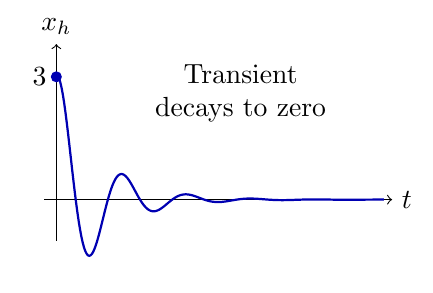
\begin{tikzpicture}[x=0.52cm,y=0.52cm]
    \path[use as bounding box] (-0.7,-1.6) rectangle (8.5,4.2);

    \draw[->] (-0.3,0) -- (8.2,0) node[right] {$t$};
    \draw[->] (0,-1) -- (0,3.8) node[above] {$x_h$};

    \draw[blue!70!black,thick,domain=0:8,samples=250]
        plot (\x,{exp(-\x)*(3*cos(deg(4*\x))+sin(deg(4*\x)))});

    \fill[blue!70!black] (0,3) circle (2pt);
    \node[left] at (0,3) {$3$};

    \node[align=center] at (4.5,2.6)
        {Transient\\decays to zero};
\end{tikzpicture}

\small (a) $x_h(t)=e^{-t}(3\cos t+\sin t)$
\end{minipage}
\hfill
%-------------------- Full solution --------------------
\begin{minipage}[t]{0.48\linewidth}
\centering
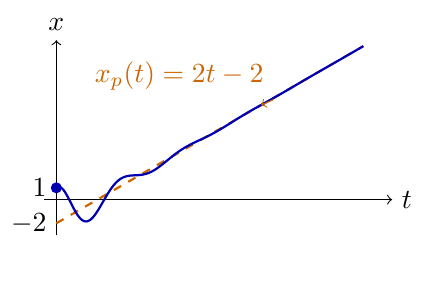
\begin{tikzpicture}[x=0.52cm,y=0.15cm]
    \path[use as bounding box] (-0.7,-5.55) rectangle (8.5,14.56);

    \draw[->] (-0.3,0) -- (8.2,0) node[right] {$t$};
    \draw[->] (0,-3) -- (0,13.5) node[above] {$x$};

    % Steady-state response
    \draw[orange!80!black,dashed,thick,domain=0:7.5]
        plot (\x,{2*\x-2});

    % Full solution
    \draw[blue!70!black,thick,domain=0:7.5,samples=250]
        plot (\x,{
            exp(-\x)*(3*cos(deg(4*\x))+sin(deg(4*\x)))
            +2*\x-2
        });

    \fill[blue!70!black] (0,1) circle (2pt);
    \node[left] at (0,1) {$1$};
    \node[left] at (0,-2) {$-2$};

    \node[orange!80!black,align=center] (steady) at (3,10.5)
        {$x_p(t)=2t-2$};
    \draw[->,orange!80!black] (steady.south east) -- (5,8);
\end{tikzpicture}

\small (b) $x(t)=x_h(t)+x_p(t)$
\end{minipage}
\caption{The transient decays, leaving the steady-state
response to describe the long-term motion.
The panels use different vertical scales.}
\end{figure}

Here, ``steady-state'' does not mean constant. The force
continues to increase, so the long-term displacement
increases as well. Next time, we will study periodic forcing. We will see how
the forcing frequency, the spring's natural frequency,
and damping affect the response, including the phenomena
of \textbf{beats} and \textbf{resonance}.


\end{document}
